\documentclass[journal=iecred,manuscript=article]{achemso}

\usepackage{color}
\usepackage{tocloft}
\cftpagenumbersoff{figure}
\setlength{\parskip}{0.25\baselineskip}
\renewcommand*{\bibfont}{\large}
\usepackage{times}
\usepackage{graphicx}
\renewcommand{\listfigurename}{Captions for Figures}
\usepackage{threeparttable}
\usepackage{wrapfig}
\usepackage{siunitx}
\usepackage{color}
\usepackage{epsf}
\usepackage{booktabs}
\usepackage{lipsum}
\usepackage{enumitem}
\linespread{1.2}

\author{Yang Xiao and Arvind Varma}

\affiliation[Purdue University]
            {Davidson School of Chemical Engineering, Purdue University, West Lafayette, IN 47907-2100}
            \email{avarma@purdue.edu}
            \phone{765-494-8484}
            \fax{765-494-0805}
            \title[An \textsf{achemso} demo]
                  {Kinetics of Glycerol Conversion to Hydrocarbon Fuels over Pd/H-ZSM-5 Catalyst}

                  

\begin{document}


\newpage
\section{Abstract}

The utilization of glycerol, primary byproduct of biodiesel production, is important to enhance process economics.
In our recent prior work, it was shown that glycerol can be converted to hydrocarbon fuels over bifunctional catalysts,
containing a noble metal supported on H-ZSM-5. Over Pd/H-ZSM-5 catalyst,
an optimal $\sim$60\% yield of hydrocarbon fuels was obtained.
In the present work, based on experimental data over Pd/H-ZSM-5 catalyst,
a lumped reaction network and kinetic model are developed.
Using differential kinetic experiments over the temperature range 300-450 $^{\circ}$C,
the rate constants, reaction orders and activation energies are obtained for each reaction step.
The predicted values match well with experimental data for glycerol conversion up to $\sim$90\%.

\section{Keywords}

Glycerol, Kinetics, Bifunctional Catalyst, Aromatization, Hydrodeoxygenation



\newpage
\section{Introduction}

\setlength{\parindent}{2em}
With the growing demand for renewable energy sources in recent years,
biofuels have emerged as promising alternatives to fossil fuels.
In this context, in addition to being an energy source, biodiesel also plays an important role in decreasing the global CO$_2$ footprint
\cite{Xue2011}.
As reported recently, biodiesel from soy oil can result in 57\% reduction of greenhouse gases as compared to petroleum diesel,
while the corresponding decrease using waste grease is 86\%.
\cite{EPA2010, Al_Mulali2015, Kralova2010}.

In biodiesel manufacture, about 10 wt\% crude glycerol is generated as an undesired byproduct.
The enormous increase in global production of biodiesel has resulted in a large surplus and low price of crude glycerol,
which was about 1 cent per lb at the end of 2014\cite{Ardi2015, Kong2016}.
To enhance biodiesel industry economics, therefore, it is important to utilize the byproduct crude glycerol
\cite{Thanh2012, Garlapati2016},
for which the purification process is typically employed as the initial step.  There are several methods for this step, including a universal procedure described recently which can purify crude glycerol from a variety of biodiesel plants yielding essentially pure glycerol
\cite{Xiao2013}.

Hydrocarbon fuels, including gasoline and diesel, provide high energy density and ease of transportation, playing an important role in the current global energy supply. With its current cheap and ready availability, conversion of glycerol to hydrocarbon (GTH) fuels would increase the economic value of glycerol and provide an additional bioenergy source.
In our recent work \cite{Xiao2016},
bifunctional catalysts (Pt/H-ZSM-5 and Pd/H-ZSM-5) were selected, prepared, characterized, and tested for GTH conversion.
Under optimal conditions, about 90\% glycerol conversion and 60\% yield of aromatic hydrocarbons were achieved over Pd/H-ZSM-5 catalyst.
A mechanism of sequential hydrodeoxygenation and aromatization was proposed for GTH conversion.
Similar works, using catalysts such as PdO/H-ZSM-5, Zn/H-ZSM-5 and Sn/H-ZSM-5, have also been reported
\cite{Hoang2010, Jang2014, Xiao2015b, Tamiyakul2015, Wang2016}.

The GTH conversion is a complex process, involving more than 20 species,
such as acetaldehyde, propenal (acrolein), hydroxyacetone, ethylene and C$_6$-C$_8$ aromatic hydrocarbons.
The reaction pathways, including dehydration, dehydrogenation/hydrogenation and oligomerization, have been proposed
\cite{Tamiyakul2015, Wang2016}.
To our knowledge, however, kinetic studies of GTH conversion have not been reported previously.
For such complex reaction networks, containing a large number of chemical species,
lumped kinetic models are typically developed to represent the overall reaction pathways \cite{Nace1971, Jacob1976, Astarita1988, Keipert1995, Ranzi2001, Olcese2013},
which can be further used for reactor design and process scale-up. 
In the present study, based on our prior work \cite{Xiao2016},
differential kinetic experiments of GTH conversion are reported,
a lumped kinetic model is developed, and reaction mechanism is discussed.


\section{Experimental}

\subsection{Materials, Catalyst Preparation and Characterization}

Palladium (II) nitrate hydrate (99.8\%  metals  basis), from Alfa  Aesar, was used as the Pd metal precursor.
ZSM-5 (Si/Al=40) of ammonium form was supplied by Zeolyst International.
Pure glycerol (ACS grade) and 37 wt\% HCl were obtained from Mallinckrodt Chemicals.
The chemical standards, including acetaldehyde, benzene, cumene, ethylene, hydroxyacetone, propanal, acrolein, propylene, toluene,
m-xylene, o-xylene and p-xylene, were from Sigma Aldrich.
Ultrahigh purity grade gases (H$_2$, He, O$_2$, N$_2$ etc.) were purchased from Indiana Oxygen. 

The ammonium form of ZSM-5 (Si/Al=40) was converted to its H-form (H-ZSM-5) by calcining in air at 500 $^{\circ}$C for 4 hours. \cite{Chiang2010, Iorio2015}
The catalyst was prepared by impregnation method.
Briefly, Pd precursor was dissolved in deionized water, and added dropwise to the well stirred H-ZSM-5 slurry,
with pH=5.6 and stirring continued for at least 8 hours at room temperature.
The slurry was then rinsed and dried in air at 100 $^{\circ}$C.
The Pd loading was 5 wt\%.
In later sections, metal loading and Si/Al ratio in H-ZSM-5 are not noted explicitly when describing the catalyst.
Thus, Pd/H-ZSM-5 refers to 5 wt\% Pd loaded on H-form of ZSM-5 with a Si/Al ratio of 40.

Since the same Pd/H-ZSM-5 catalyst, as in our prior publication \cite{Xiao2016},
was used in the present work, results of catalyst characterization, including BET specific surface area, mean pore diameter, Pd metal dispersion (by H$_2$-O$_2$ titration \cite{Benson1965}),
Pd particle size, AEC-ICP element analysis, NH$_3$-TPD, transmission electron microscopy (TEM), X-ray photoelectron spectroscopy (XPS) and X-ray powder diffraction (XRD), can be found in that publication and its Supplementary Information.
Briefly, the high BET surface area (437 m$^2$/g) and moderate mean pore diameter (about 0.5 nm) of Pd/H-ZSM-5 indicates good accessibility of reactants (e.g. glycerol, acrolein and olefin gases) over Pd/H-ZSM-5 catalysts.
Both surface area and mean pore diameter data are consistent with those reported in the literature. \cite{Serrano-Ruiz2011, Olson1981}
The Pd particle sizes provided by TEM (3.8 nm) and H$_2$-O$_2$ titration (3.2 nm) techniques are consistent, corresponding to Pd metal dispersion of 23-30\%.
The XRD patterns for Pd/H-ZSM-5 are similar to unsupported MFI (ZSM-5), as reported in the International Zeolite Association (IZA) structure database. \cite{Baerlocher2007}
No Pd peaks were identified, likely due to high metal dispersions and low metal loading \cite{Zhu2013}.
The NH$_3$-TPD measurements showed a Br{\o}nsted acid peak at about 650 K \cite{Iorio2015}.


\subsection{Kinetic Measurements and Product Analysis}

The experiments were conducted in a continuous fixed-bed reactor system,
described in our prior work. \cite{Xiao2016}
The catalysts were packed in a stainless steel fixed-bed reactor (with internal diameter 10 mm).
Prior to kinetic measurements, 
catalysts were activated at 400 $^{\circ}$C, 1 atm for 4 h under a gas mixture  (25\% H$_2$, 75\% N$_2$) flow.
Feedstocks were heated to their boiling points to ensure evaporation prior to being pumped by an IP 25 Isocratic pump from Dionex into the reactor.
The product mixture was condensed in a dual-wall glass condenser, cooled by propanediol circulation (to -20 $^{\circ}$C) controlled by a circulator (Thermo Haake C10).
The liquid products were collected every 10 min and then analyzed,
while the gaseous products were analyzed on-line every 5 min.
The standard operating conditions were 400 $^{\circ}$C, 1 atm total pressure,
0.05 g catalyst, mixed gas of N$_2$ and H$_2$ at flow rates 100 mL/min and 50 mL/min respectively,
and pure glycerol feed rate 0.6 mL/h (liquid, at room temperature).
Based on the standard operating procedure, to obtain kinetic data under various conditions, parameters including temperature, reactant feed flow, catalyst packing amount were varied.
All experiments were conducted under excess hydrogen flow (feed molar ratio of H$_2$ to glycerol $\sim$ 10).
A blank test with packing inert material (amorphous SiO$_2$), instead of Pd/H-ZSM-5, was conducted under the standard reaction conditions.
It was found that glycerol conversion was $<$ 1\%.
All experiments have mass balances of 90 $\pm$ 3\%,
consistent with the literature \cite{Jongerius2013}.
Possible factors affecting mass balance include liquid hold-up in the reactor, condenser and tubing.
All kinetics measurements were conducted under differential conditions, corresponding to 5-10 \% conversion.
All experiments were repeated at least twice.
        
The products from GTH process split into three phases: non-condensable gaseous, upper organic liquid and lower aqueous liquid, 
which were analyzed by three different instruments.
The gases were analyzed by a micro-GC (Agilent 3000A) equipped with a thermal conductivity detector, a Mol-Sieve 5A column and a Plot U column.
The organic liquid products were analyzed by an Agilent GC 6890 equipped with flame ionization detector (FID) and a DB-WAX (30 m $\times$ 0.32 mm) column,
while the aqueous liquid samples were analyzed by an Agilent GC 5890 equipped with a FID and Select Biodiesel for glycerides ultiMetal Column (15m $\times$ 0.32 mm, ID=0.10 mm) and a retention gap. 
Calibration was performed for all the components. 


\section{Results and Discussion}

\subsection{Proposed Reaction Pathways}

As described in our prior work \cite{Xiao2016},
oxygenates (acrolein, acetol, etc.) were primary products when unsupported H-ZSM-5, Pd/SiO$_2$ (amorphous) and Pt/SiO$_2$ (amorphous) were used as catalysts,
although the use of H-ZSM-5 promoted the formation of target products, aromatic hydrocarbon fuels.
The addition of noble metal Pd to H-ZSM-5, as compared to unsupported H-ZSM-5,
enhanced yield towards aromatics and decreased the selectivity to oxygenates (see \ref{T_products}),
where selectivity of a component refers to the production rate of that component per unit consumption rate of glycerol.
In our prior work, the metal and acidity of ZSM-5 effects were discussed.
Briefly, it was concluded that GTH conversion follows sequential hydrodeoxygenation (HDO) and aromatization steps,
promoted by metals (Pd or Pt) and acidic H-ZSM-5 support.
Thus, surface Pd and acidic sites of H-ZSM-5 are proposed as the active sites.
The operating conditions, including temperature, H$_2$ partial pressure, glycerol feed flow rate and catalyst packed amount,
were also varied and optimized in our prior work.
The optimized parameters were used as the standard conditions in the present work. 

Since the only carbon containing species in the feed was glycerol,
all three carbon containing products (oxygenates, gases and aromatics) derived from it.
As shown in \ref{F_network}, the partially deoxygenated products, oxygenates,
are proposed as intermediates resulting in the fully deoxygenated products - gases and aromatics, as also suggested by others \cite{Tamiyakul2015, Wang2016}.
This leads to the proposed steps R1, R2 and R3.
Further, as reported in the literature \cite{Kitagawa1986, Ono1992, Choudhary2001},
gases can be converted over ZSM-5 type zeolites to aromatics, thus step R4 is included in the reaction network.
In summary, oxygenates are first formed from glycerol (step R1),
followed by formation of aromatics either directly (step R3) or indirectly via gases (steps R2 and R4).

\subsection{Absence of Mass and Heat Transfer Effects}

Before conducting the kinetic measurements, using well known procedures,
the plug flow condition was confirmed by satisfying the criteria proposed previously \cite{Perego1999}.
Specifically, the reactor diameter is more than 10 times the catalyst particle diameter,
while the catalyst bed height is more than 50 times the catalyst particle diameter.
The absence of internal/external mass transfer limitations was also confirmed (\ref{F_transfer}).
By varying only packed catalyst particle diameter ($d_{p}$) in the range 100 micron $<$ $d_{p}$ $<$ 1000 micron,
\ref{F_transfer}(a) was obtained.
It shows that when $d_{p}$ $<$ 150 micron (corresponding to 100 mesh), internal mass transfer effect was negligible.
\ref{F_transfer}(b) was obtained by varying feed flow rate, while keeping other operating conditions, including contact time (W/F), unchanged.
It indicates that for feed flow rate $>$ 0.4 mL/h, no significant external mass transfer effect exists.
Thus, $d_{p}$ $<$ 150 micron and feed flow rate $>$ 0.4 mL/h were used in the kinetic experiments.
Further, the criteria by Weisz and Prater \cite{Weisz1954}
$\left(\frac{d^2_pr_i\rho_{cat}}{C_iD_{eff}}  < 1\right)$
and Mears \cite{Mears1971}
$\left(\frac{r_i \Delta H_i \rho_{cat} d_p E_{a_{i}} }{h R T^2} < 0.15\right)$
were both satisfied as well, confirming the absence of mass and heat transfer effects in all measurements.

\subsection{Kinetic Model Development}

In the reaction pathways shown in \ref{F_network}, each step (R1-R4) contains more than one elementary reaction.
For example, step R1, when converting glycerol to acrolein,
involves two sequential dehydration reactions \cite{Gu2012, Zhang2015, Galadima2016b},
while more complex reactions (e.g. hydrogenation, dehydrogenation, deoxygenation, etc.)
occur when other oxygenates are produced \cite{Park2015, Tamiyakul2015, Wang2016}.
Step R2 includes deoxygenation, dehydrogenation and C-C bond cleavage reactions,
while step R4 includes oligomerization, cyclization and dehydrogenation.
Step 3 refers to pathways where C$_1$-C$_3$ gases do not exist.
Thus the overall GTH conversion comprises a complex network,
which can be reduced to a few equivalent lumped reactions: steps R1-R4.
As lumped pseudo-components, oxygenates represent a mixture of acetaldehyde, propanal, acrolein and hydroxyacetone.
Gases represent a mixture of methane, ethylene and propylene, while aromatics refer to C$_6$-C$_{12}$ aromatic hydrocarbons.

The reaction rate of step Ri is defined by Eq. (\ref{Eq1}).

\begin{equation} \label{Eq1}
r_i=\frac{dF_i}{dW}
\end{equation}


Since all kinetic measurements, as described in the experimental section,
were conducted under differential operating conditions (conversion 5-10\%),
the reaction rate is calculated by Eq. (\ref{Eq3}).

\begin{equation} \label{Eq3}
r_i=F_{0} \times \frac{X_i}{W}
\end{equation}

The consumption/formation rates of glycerol and lumped components (oxygenates, gases and aromatics) are given by Eqs. (\ref{Eq4} -~\ref{Eq7}).

\begin{equation} \label{Eq4}
\frac{dF_{GLY}}{dW}=-r_1
\end{equation}
\begin{equation} \label{Eq5}
\frac{dF_{OXY}}{dW}=r_1-r_2-r_3
\end{equation}
\begin{equation} \label{Eq6}
\frac{dF_{GAS}}{dW}=r_2-r_4
\end{equation}
\begin{equation} \label{Eq7}
\frac{dF_{ARO}}{dW}=r_3+r_4
\end{equation}

Note that among the four Eqs. (\ref{Eq4} -~\ref{Eq7}), only three are independent.
An overall material balance yields the following Eqs. (\ref{Eq8} -~\ref{Eq10}).

\begin{equation} \label{Eq8}
F_{GLY}+F_{OXY}+F_{GAS}+F_{ARO}=F_{0}
\end{equation}
\begin{equation} \label{Eq10}
P_{i}=F_{i} \times \frac{P_{0}}{F_{0}}
\end{equation}


\subsection{Glycerol to Oxygenates (Step R1)}

Since excess H$_2$ (molar ratio of H$_2$ to glycerol $\sim$10) is used in all cases,
H$_2$ pressure effect was considered as a constant contribution to the reaction rates.
Kinetic measurements were carried out at various temperatures in the range 300-450 $^{\circ}$C.
Although only results at 400 $^{\circ}$C are shown below, since it gives optimum aromatic yields \cite{Xiao2016},
fitting results for other temperatures gave essentially the same conclusions.

When glycerol was fed as reactant,
under differential operating conditions,
all lumped components (oxygenates, gases and aromatics) were detected.
By varying glycerol feed flow rate,
its consumption rate corresponding to its average bed partial pressure,
was measured, as shown and fitted in \ref{F_glycerol}.

Being the first step of the network,
the consumption rate of glycerol depends only on glycerol partial pressure.
Since a linear fit works well,
step R1 appears to be first-order,
which is consistent with the literature \cite{Akizuki2012, Talebian-Kiakalaieh2014, Park2015, Talebian-Kiakalaieh2015}.
Thus, Eq. (\ref{Eq4}) can be rewritten as Eq. (\ref{Eq11}).

\begin{equation} \label{Eq11}
-\frac{dF_{GLY}}{d_{W}}=r_1=k_1 P_{GLY}
\end{equation}

From slope of the line in \ref{F_glycerol}, the value of $k_1$ at 400 $^{\circ}$C is 0.278 $mol/(g_{cat} \cdot h \cdot atm)$.

\subsection{Oxygenates as Reactant (Steps R2 and R3)}

In the above section, the rate constant and reaction order of step R1 were obtained by feeding glycerol in a differential reactor,
controlling its conversion in the range 5-10\%.
To study the rate constants and reaction orders of steps R2-R4,
still under differential operating conditions,
oxygenates were used as feed.
The oxygenates, based on the compositions reported in our prior work \cite{Xiao2016},
were represented by a mixture of acetaldehyde, propanal, acrolein and acetol.
Because acrolein was found to be the primary component (60-93\%), pure acrolein was also tested as feed.
As shown in \ref{F_oxygenates}, both pure acrolein and oxygenates curves show good second-order fits,
while formation rates of gases and aromatics, corresponding to  $r_2$-$r_4$ and $r_3$+$r_4$ respectively, appear to be second-order as well.

The conversion of acrolein to gases likely includes hydrogenation of acrolein to propanol, followed by propanol dehydration and other C-C cleavage reactions.
 \cite{Marinelli1995, Mohr2000, Volckmar2009}.
Both first and second orders have been reported for acrolein hydrogenation\cite{Jesus1999, Wei2013}.
Since reaction rates starting with representative oxygenates and pure acrolein as feed, as shown in \ref{F_oxygenates}, are close,
only pure acrolein was used for further kinetic measurements, discussion and analysis.

Both gases and aromatics were detected when oxygenate conversions were lower than 10\%.
Since no glycerol was fed ($r_1$=0), the consumption rate of oxygenates is dependent only on $r_2$ and $r_3$,
as described by Eq. (\ref{Eq5}).
\ref{F_oxygenates} shows that the overall reaction rates of $r_2$ + $r_3$ follow a second-order.
It is assumed here (justified later) that reaction orders of steps R2 and R3 are the same, thus $n_2$=$n_3$=2.
Eq. (\ref{Eq5} -~\ref{Eq7}) are then rewritten as Eq. (\ref{Eq12} -~\ref{Eq15}).

\begin{equation} \label{Eq12}
-\frac{dF_{OXY}}{dW}=r_2+r_3=(k_2+k_3)P_{OXY}^2
\end{equation}

\begin{equation} \label{Eq14}
\frac{dF_{GAS}}{dW}=r_2-r_4=k_2P_{OXY}^2-k_4P_{GAS}^{n_4}
\end{equation}

\begin{equation} \label{Eq15}
\frac{dF_{ARO}}{dW}=r_3+r_4=k_3P_{OXY}^2+k_4P_{GAS}^{n_4}
\end{equation}

To determine reaction order of step R4 ($n_4$) and all rate constants ($k_2$-$k_4$), 
Eq. (\ref{Eq16}) is obtained dividing Eq. (\ref{Eq15}) by Eq. (\ref{Eq14}):


\begin{equation} \label{Eq16}
\frac{dF_{ARO}}{dF_{GAS}}=\frac{k_3 P_{OXY}^2+k_4 P_{GAS}^{n_4}}{k_2 P_{OXY}^2-k_4 P_{GAS}^{n_4}}=\alpha
\end{equation}
 
In \ref{F_234}(a),
the aromatics partial pressure is plotted versus the partial pressure of gases.
Since a linear relation fits well, $\alpha$ in Eq. (\ref{Eq16}) equals a constant.
Rearranging Eq. (\ref{Eq16}) yields Eq. (\ref{Eq17}), whose rhs also equals a constant, designated as $\beta$.

\begin{equation} \label{Eq17}
\frac{P_{GAS}^{n_4}}{P_{OXY}^2}=\frac{\alpha k_2 - k_3}{k_4(\alpha + 1)}=\beta
\end{equation}

Taking logarithm of both sides yields Eq. (\ref{Eq18}).

\begin{equation} \label{Eq18}
logP_{OXY}^2=n_4logP_{GAS}-log\beta
\end{equation}

The plot of Eq. (\ref{Eq18}) is shown in \ref{F_234}(b),
where the fitted slope is 0.968, thus step R4 is found to be first-order.

Additional tests for reaction orders of steps R2 and R3 were carried out,
such as the following data sets:
$n_2$=1, $n_3$=1; $n_2$=1, $n_3$=2; $n_2$=2, $n_3$=1;$n_2$=2, $n_3$=3; and $n_2$=3, $n_3$=2, etc.
These sets, however, always provided worse fits. Thus it is confirmed that the assumption of $n_2$=2, $n_3$=2 is reasonable.

To determine $k_2$, $k_3$ and $k_4$,
the following procedure was used. 
First, the value of ($k_2+k_3$) was obtained from Eq. (\ref{Eq12}) by the best fit of the oxygenate curve in \ref{F_oxygenates}.
A second relation between $k_2$ and $k_4$ was obtained via Eq. (\ref{Eq14}), using the measured values of the gas formation rate.
An alternative for the second relation is via Eq. (\ref{Eq15}), using the measured values of the aromatics formation rate.
The third relation between $k_2$, $k_3$ and $k_4$ was from the measured values of $\alpha$ via Eq. (\ref{Eq16}).
These three relations were used to obtain the best fit $k_2$, $k_3$ and $k_4$ values at 400 $^{\circ}$C, shown in \ref{T_all_k}.   

\subsection{Effect of Temperature} 

All data discussed in above sections was measured at 400 $^{\circ}$C,
while the reaction orders ($n_1$-$n_4$) remain the same when other temperatures (300-450 $^{\circ}$C) are used.
Reaction activation energies ($E_a$) of steps R1-R4 were calculated using the Arrhenius equation (\ref{Eq31}).
With the reaction orders remaining the same,
data for the other temperatures (300-450 $^{\circ}$C) were used to obtain the corresponding $k_i$ values.
The reaction activation energies (E$_a$) for steps (R1-R4) were then calculated by linear fits using the Arrhenius equation (Eq. \ref{Eq31}).
Good linearity was obtained for all four steps, as shown in \ref{Fitting}, and the fitted results are shown in \ref{T_Ea}. 

\begin{equation} \label{Eq31}
k_i=A_iexp\left(-\frac{E_{a_{i}}}{RT}\right)
\end{equation}

The activation energy of step R1 (glycerol dehydration to acrolein) has been reported over a wide range in the literature.
Talebian-Kiakalaieh et al. presented a value of 27.5 kJ/mol over tungstosilicic acid catalyst\cite{Talebian-Kiakalaieh2015},
while Qadariyah et al. have 39.6 kJ/mol in subcritical or supercritical water (temperature 200-400 $^{\circ}$C, pressure 30 MPa) without any catalyst \cite{Qadariyah2011}.
Watanabe et al. reported 146 kJ/mol at 300-400 $^{\circ}$C with H$_2$SO$_4$ catalyst \cite{Watanabe2007},
while Ott et al. have 140 kJ/mol at 300-360 $^{\circ}$C over zinc sulfate catalyst \cite{Ott2006}.
Our result described in \ref{T_Ea} is in the reported range of 27.5-146 kJ/mol.
The activation energy of step R2 is smaller than that of step R3 by 26 kJ/mol, 
indicating step R2 dominates in the reaction pathway as compared to step R3 (see also the relative $k_i$ values in \ref{T_all_k}).
As a series reaction, step R4, with a slightly higher activation energy, follows step R2.

With the obtained kinetic parameters,
the rates for all four steps for all the 80 experimental data points (at various temperatures, reactant feed flows and catalyst packing amounts) were calculated.
The experimental and predicted flow rates for all species are plotted in \ref{F_parity}, giving an RMS error of 6.1\%, indicating good fits.

\section{Concluding Remarks}

In the present work,
experiments were carried out for glycerol to hydrocarbon (GTH) fuels conversion over a 5 wt\% Pd/H-ZSM-5 catalyst.
Based on the data, the lumped reaction network was first established.
The differential kinetic experiments (conversion less than 10\%) were used to develop a kinetic model.
The reaction orders, rate constants and activation energies for each step in the network were determined from analysis and data fitting.
The model predicted values match well with the experimental results in the range of glycerol conversion up to 90\%.
This work provides rate expressions for the various steps involved in converting glycerol, as a biodiesel by-product, to hydrocarbon fuels.

\section{Acknowledgments}

It is a pleasure to participate in this tribute to Professor Roy Jackson.
This work was supported by the R. Games Slayter Fund.
AV also thanks the Department of Chemical Engineering,
University of California at Santa Barbara for the kind hospitality during Winter 2017 when this manuscript was completed.

\newpage

\section{Notation}

\begin{tabbing}

01\hspace*{50bp} \=02\hspace*{100bp} \=03\hspace*{50bp}\kill

$A_i$  \> $[mol/(g_{cat} \cdot h \cdot atm^{n_i})]$   \> Pre-exponential factor of step i when the reaction order is $n_i$ \\
$C_i$  \> $[mol/m^3]$   \> Concentration of species i \\
$D_{eff}$  \> $[m^2/h]$   \> Effective diffusion coefficient \\
$d_p$  \> $[m]$   \> Catalyst particle diameter \\
$E_{a_i}$  \> $[kJ/mol]$   \> Activation energy of step i \\
$F_0$  \> $[mol/h]$   \> Initial Feed flowrate \\
$F_i$  \> $[mol/h]$   \> Flowrate of species i \\
$h$  \> $[J/\left( m^2 \cdot K \cdot h\right)]$   \> Heat transfer coefficient \\
$k_i$  \> $[mol/(g_{cat} \cdot h \cdot atm^{n_i}) ]$   \> Reaction rate constant of step i when the reaction order is $n_i$\\
$n_i$  \> $[mol]$   \> Reaction order of step  i \\
$P_i$  \> $[atm]$   \> Partial pressure of species i \\
$R$  \> $[J/\left(K \cdot mol \right)]$   \> Gas constant \\
$r_i$  \> $[mol/\left( g_{cat} \cdot h\right)]$  \> Reaction rate of step i \\
$T$  \> $[K]$  \> Reaction temperature \\
$TOF_i$  \> $[h^{-1}]$  \> Turnover frequency of step i \\
$W$  \> $[g]$   \> Catalyst packing amount\\
$X_i$  \> $[-]$   \> Conversion of step  i \\
$\Delta H_i$  \> $[kJ/mol]$   \> Enthalpy change of step i \\
$\rho_{cat}$  \> $[kg/m^3]$   \> Density of packed catalyst \\


$Species:$  \>    \ \\
$GLY$  \>    \ Glycerol\\
$OXY$  \>    \ Oxygenates\\
$GAS$ \>    \ Gases\\
$ARO$  \>    \ Aromatics\\

\end{tabbing}

\newpage
\bibliographystyle{aichej}
\bibliography{Kinetics_CH4}


\newpage
\begin{center}

\listoffigures

\end{center}


\newpage
\begin{figure}[h]
  \centering
  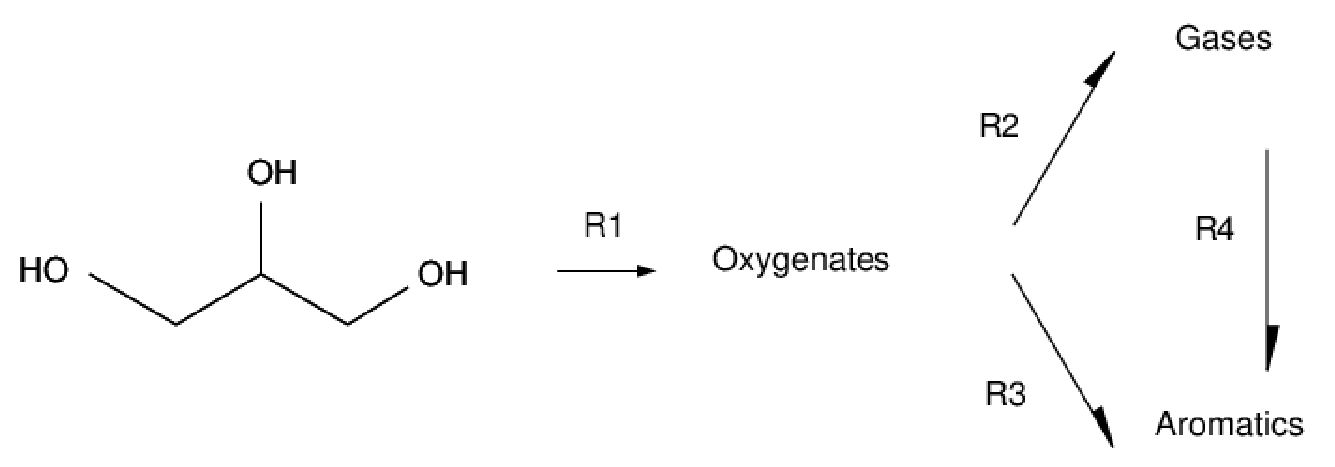
\includegraphics[width=0.85\textwidth]{Fig1.eps}
  \caption{Glycerol to Hydrocarbons (GTH) Reaction Network} \label{F_network}
\end{figure}

\newpage
\begin{figure}[!ht]
  \centering
  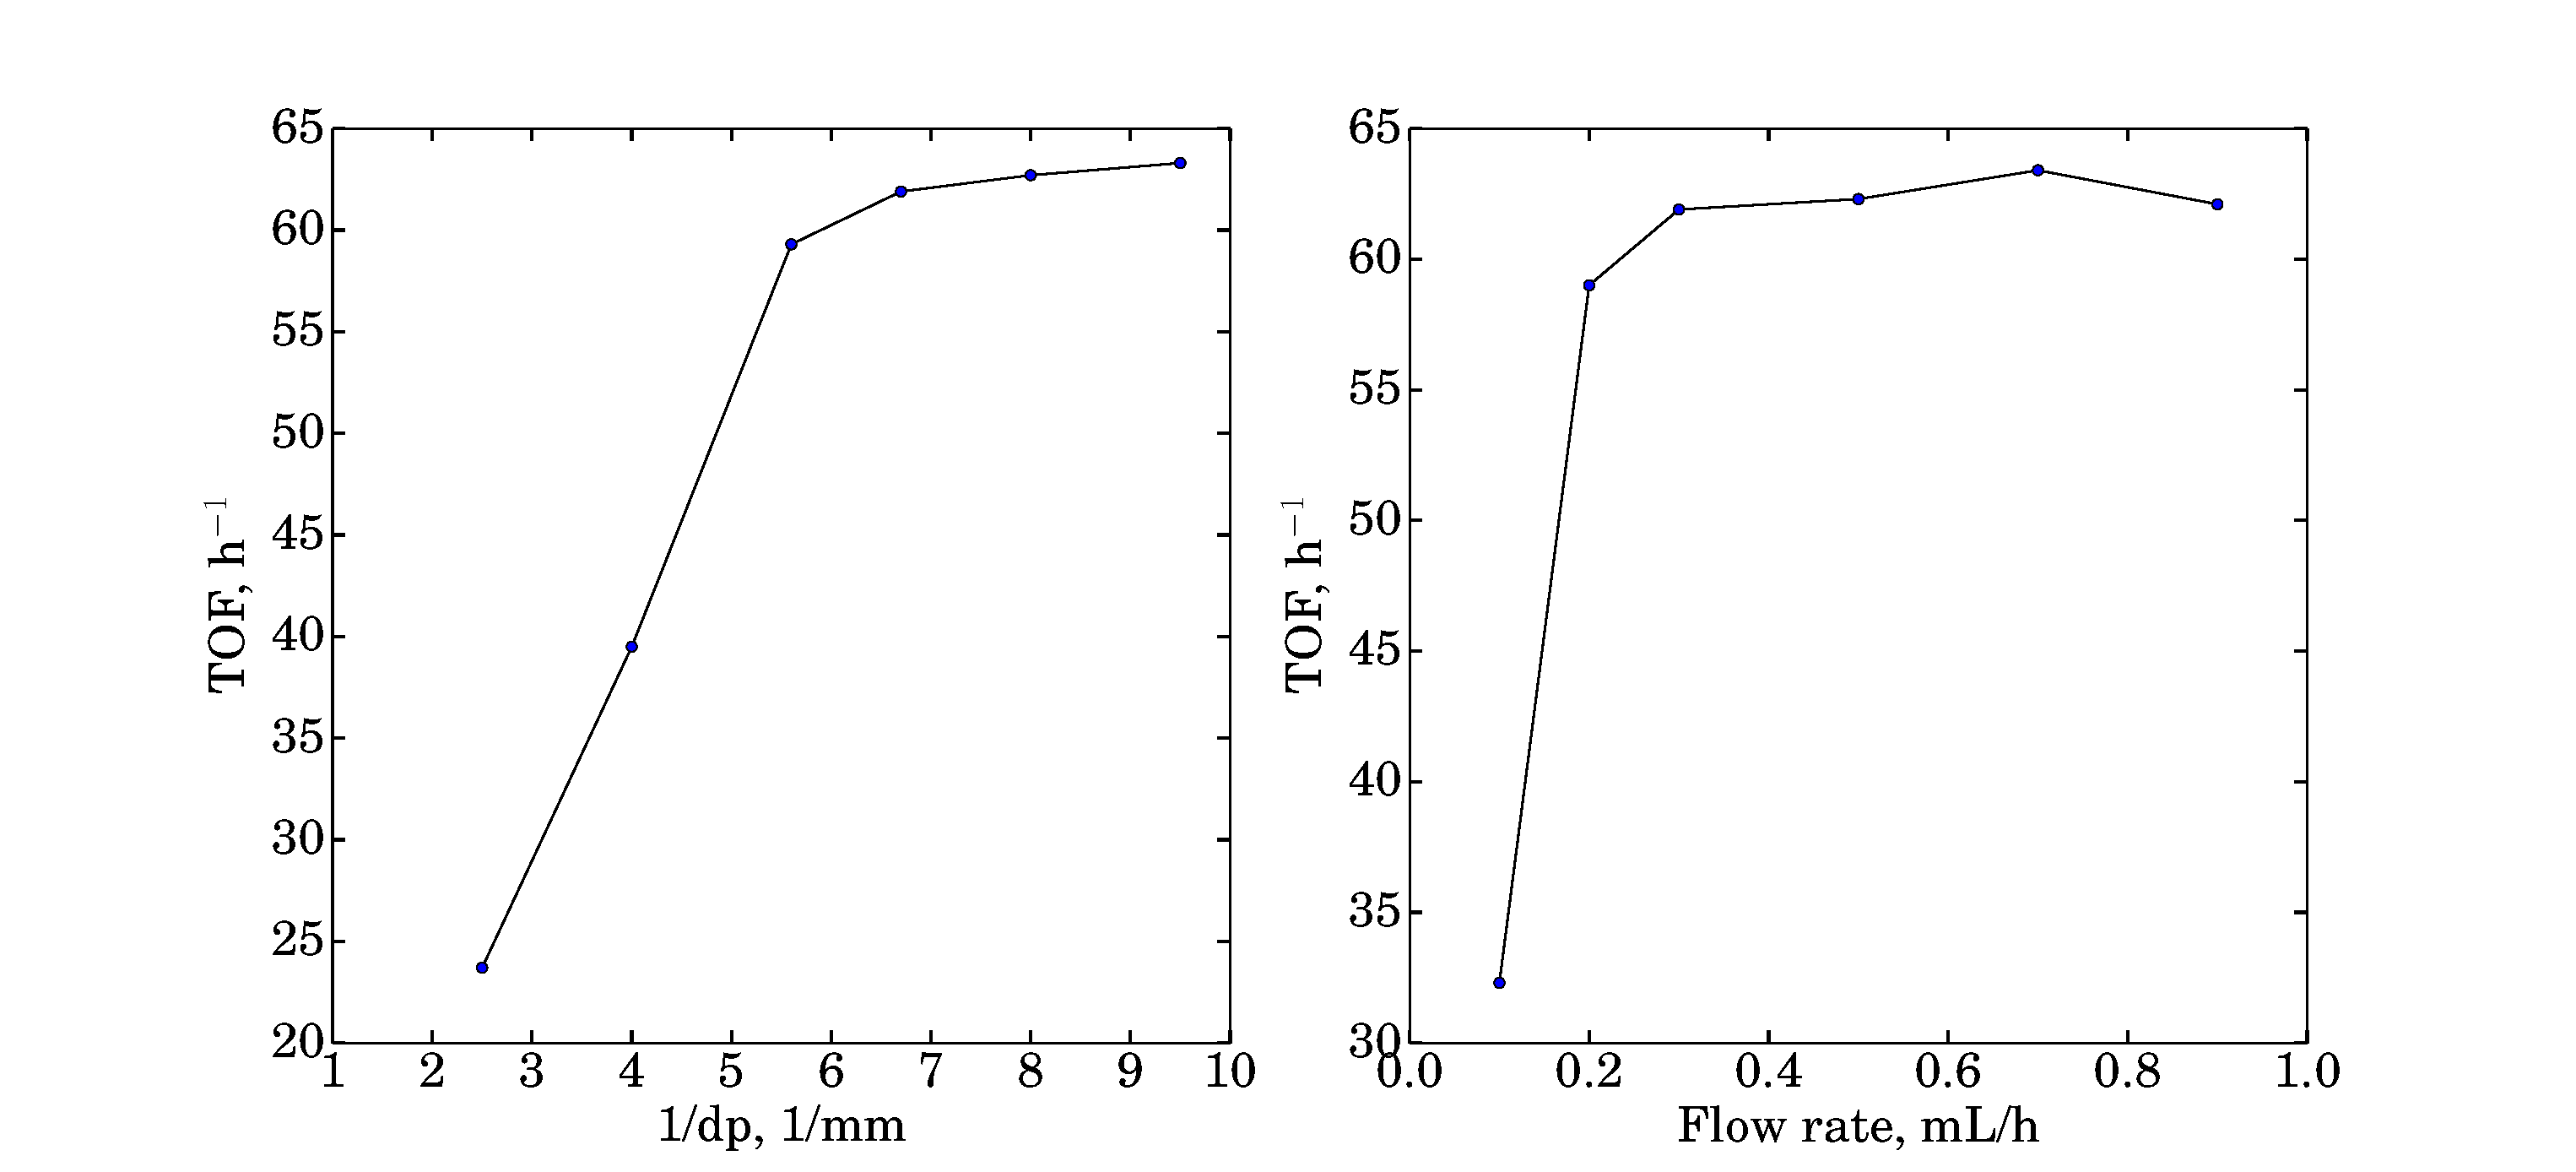
\includegraphics[width=0.85\textwidth]{Fig2.eps}
  \caption{Mass Transfer Limitation Tests for a) Internal Diffusion and b) External Diffusion}   \label{F_transfer}
\end{figure}

\newpage
\begin{figure}[!ht]
  \centering
  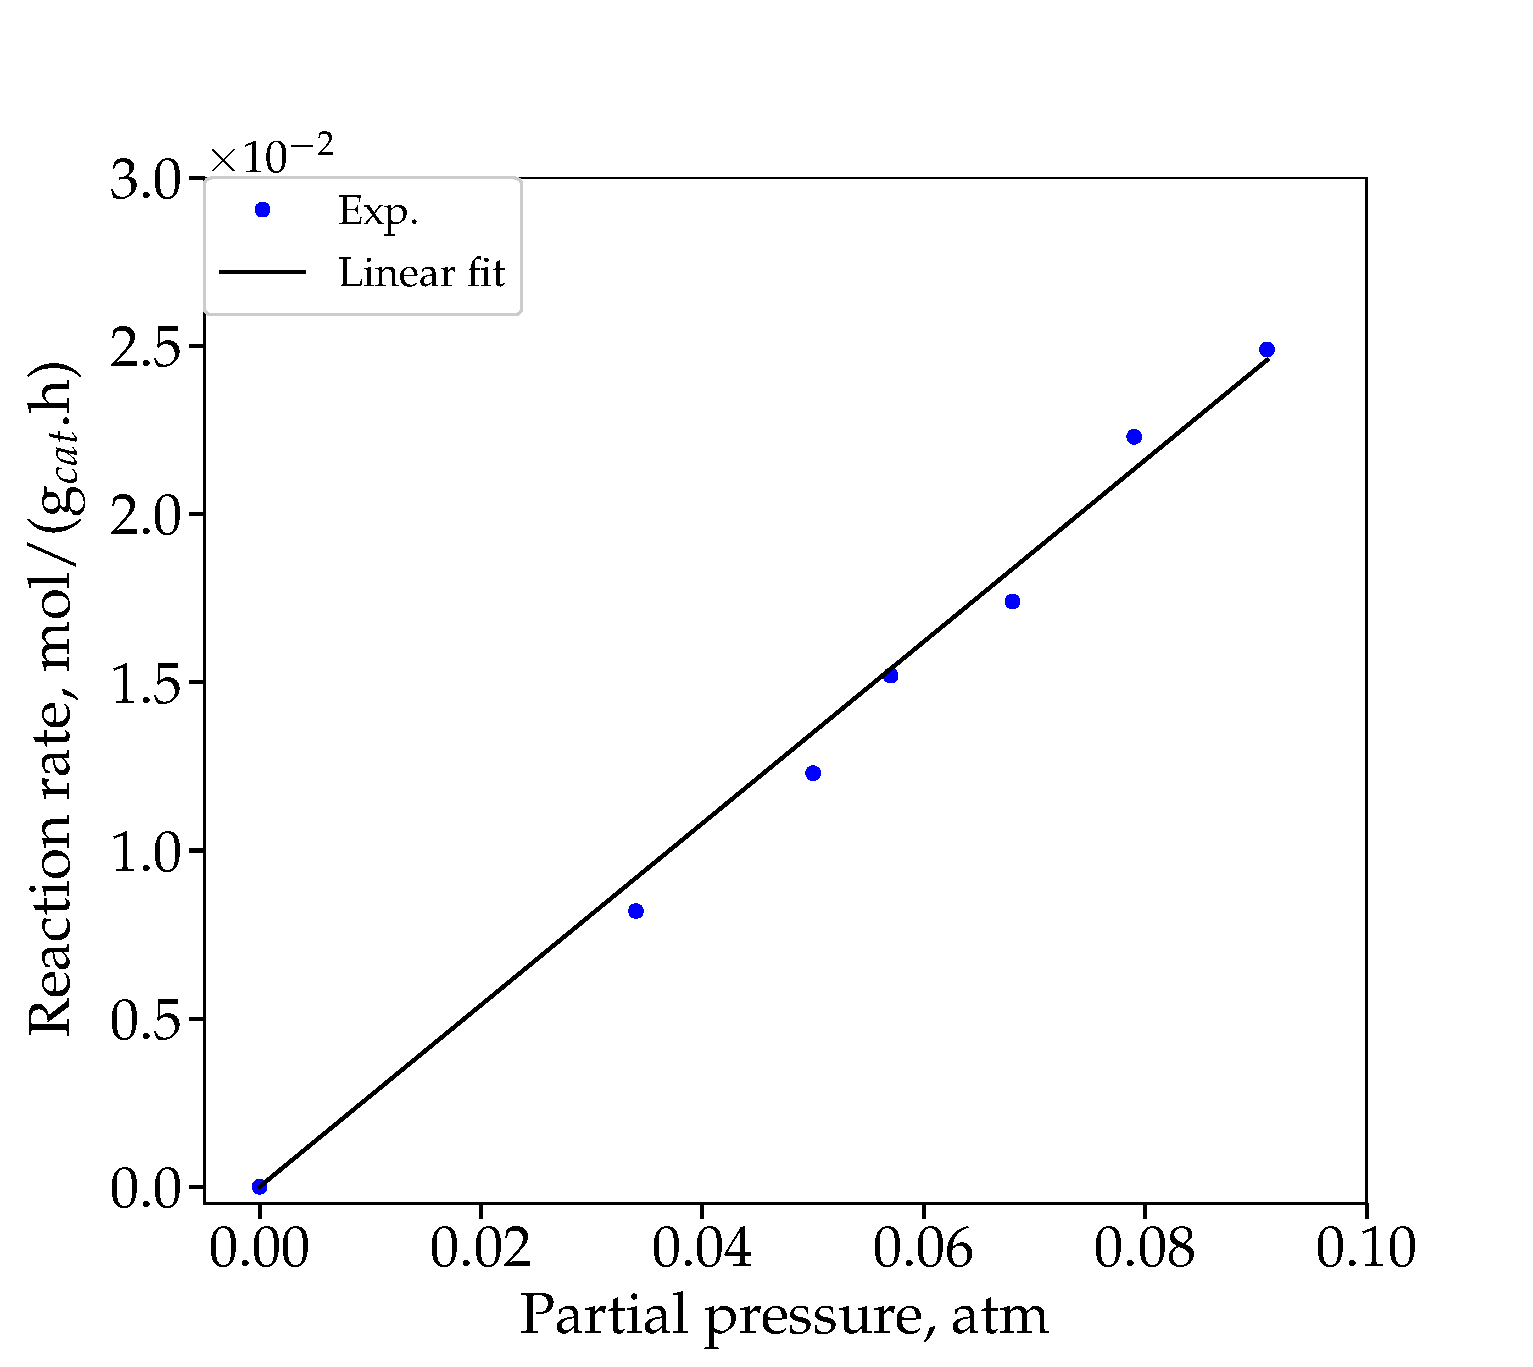
\includegraphics[width=0.85\textwidth]{Fig3.eps}
  \caption{Fit of Glycerol Reaction Rates}        \label{F_glycerol}
\end{figure}

\newpage
\begin{figure}[!ht]
  \centering
  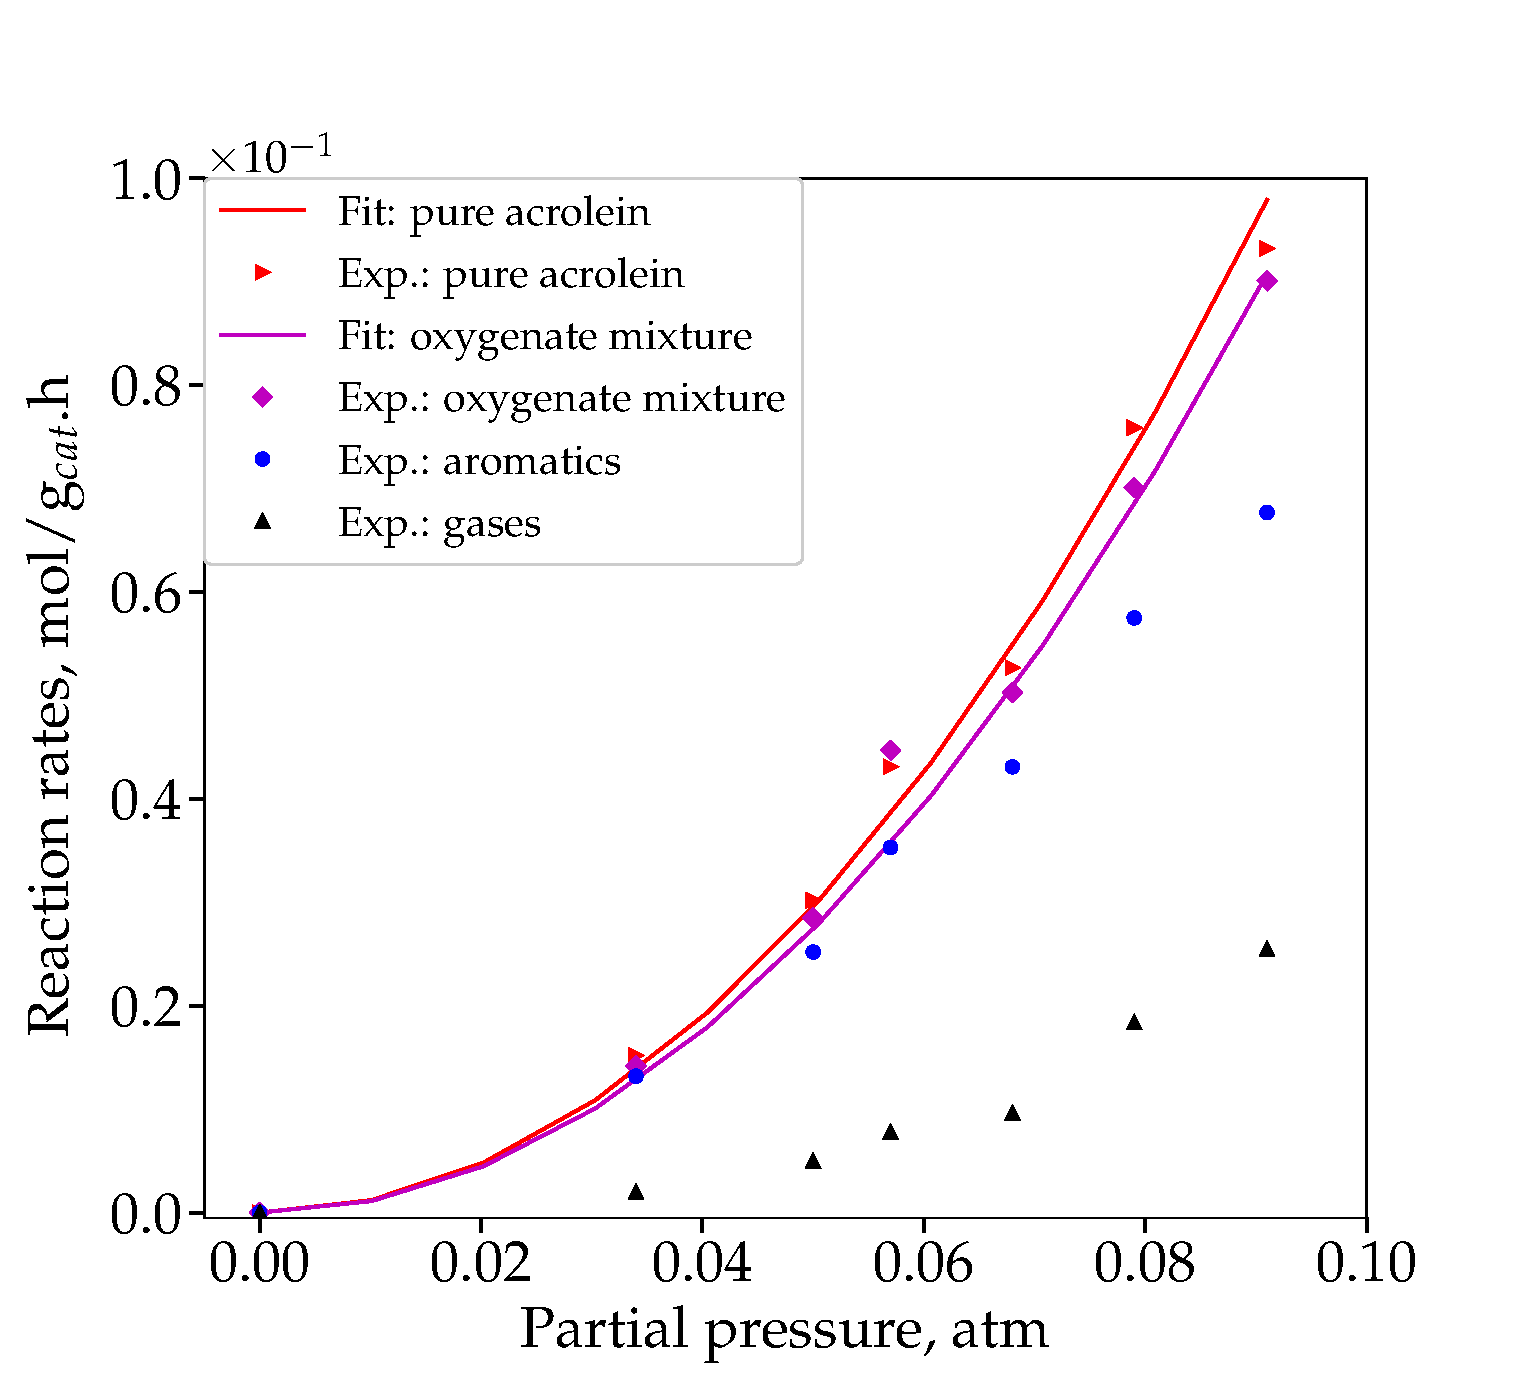
\includegraphics[width=0.85\textwidth]{Fig4.eps}
  \caption{Fit of Oxygenate Reaction Rates} \label{F_oxygenates}
\end{figure}

\newpage
\begin{figure}[!ht]
  \centering
  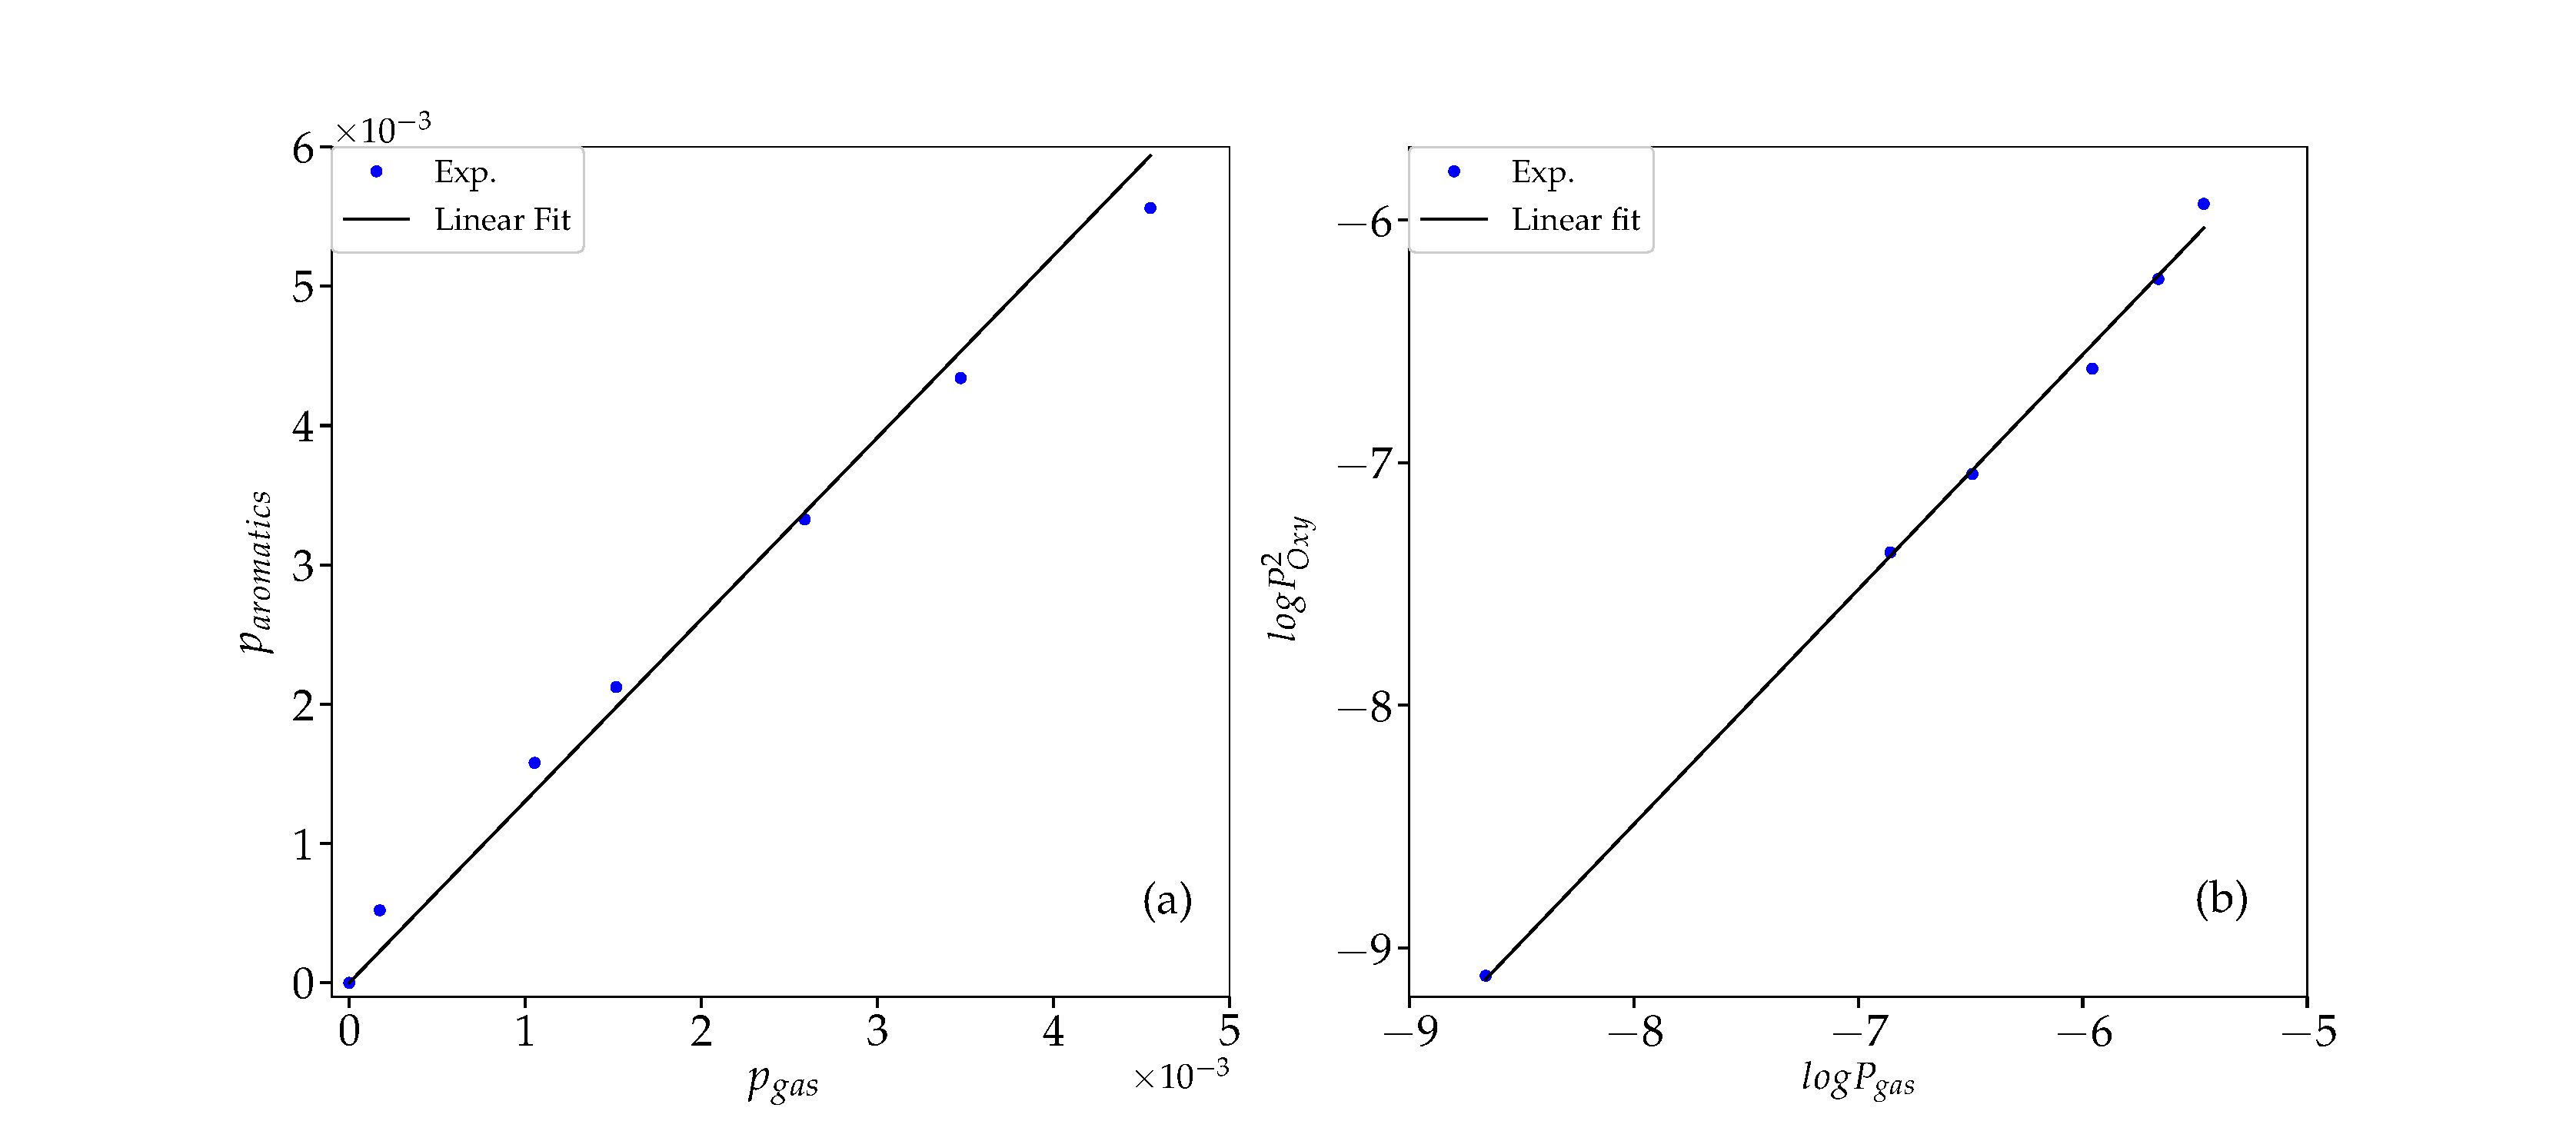
\includegraphics[width=0.98\textwidth]{Fig5.eps}
  \caption{Reaction Rate Fits of Steps R2, R3 and R4} \label{F_234}
  \end{figure}

\newpage
\begin{figure}
  \centering
  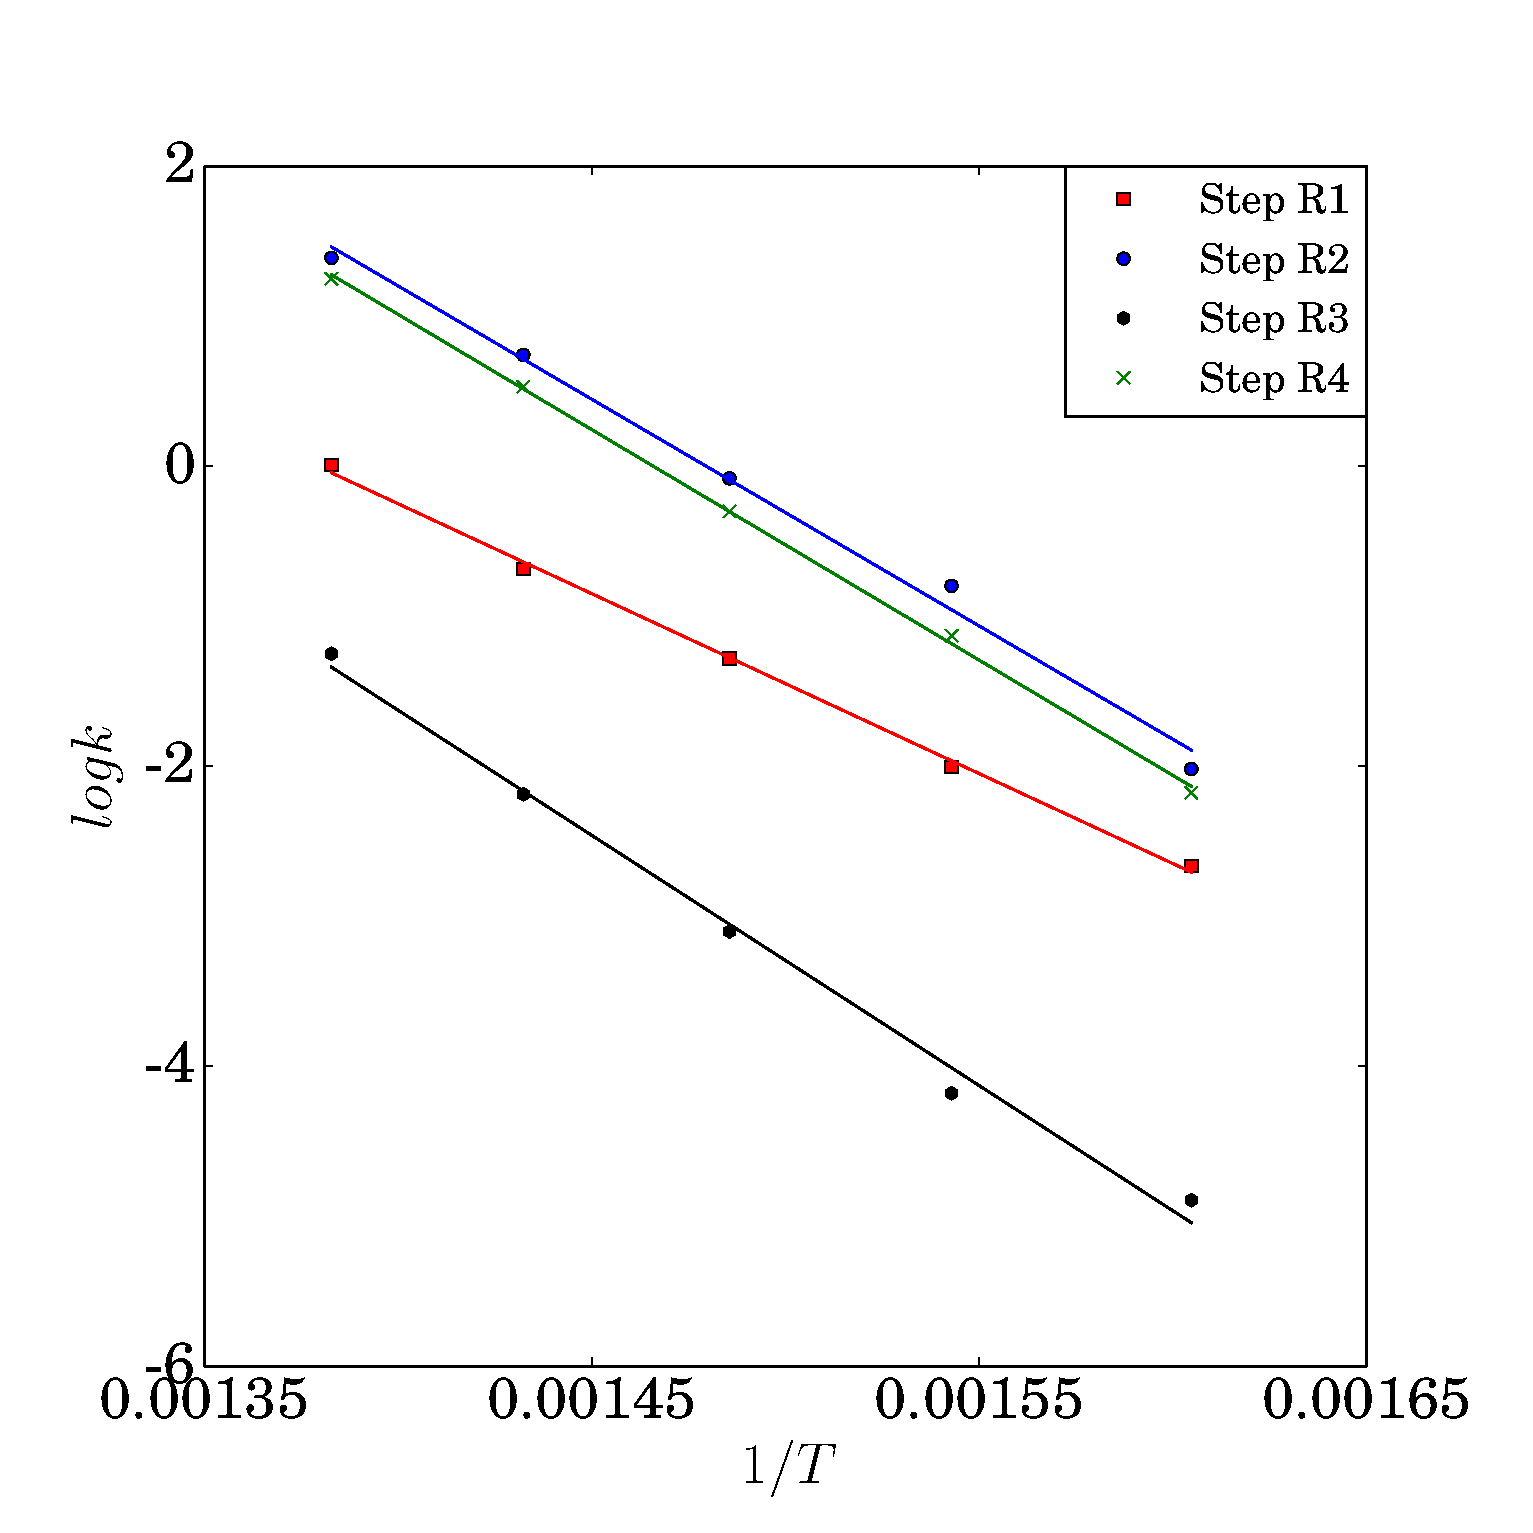
\includegraphics[width=0.85\textwidth]{Fig6.eps}
  \caption{Arrhenius Plots for the Rate Constants}  \label{Fitting}
\end{figure}

\newpage
\begin{figure}
  \centering
  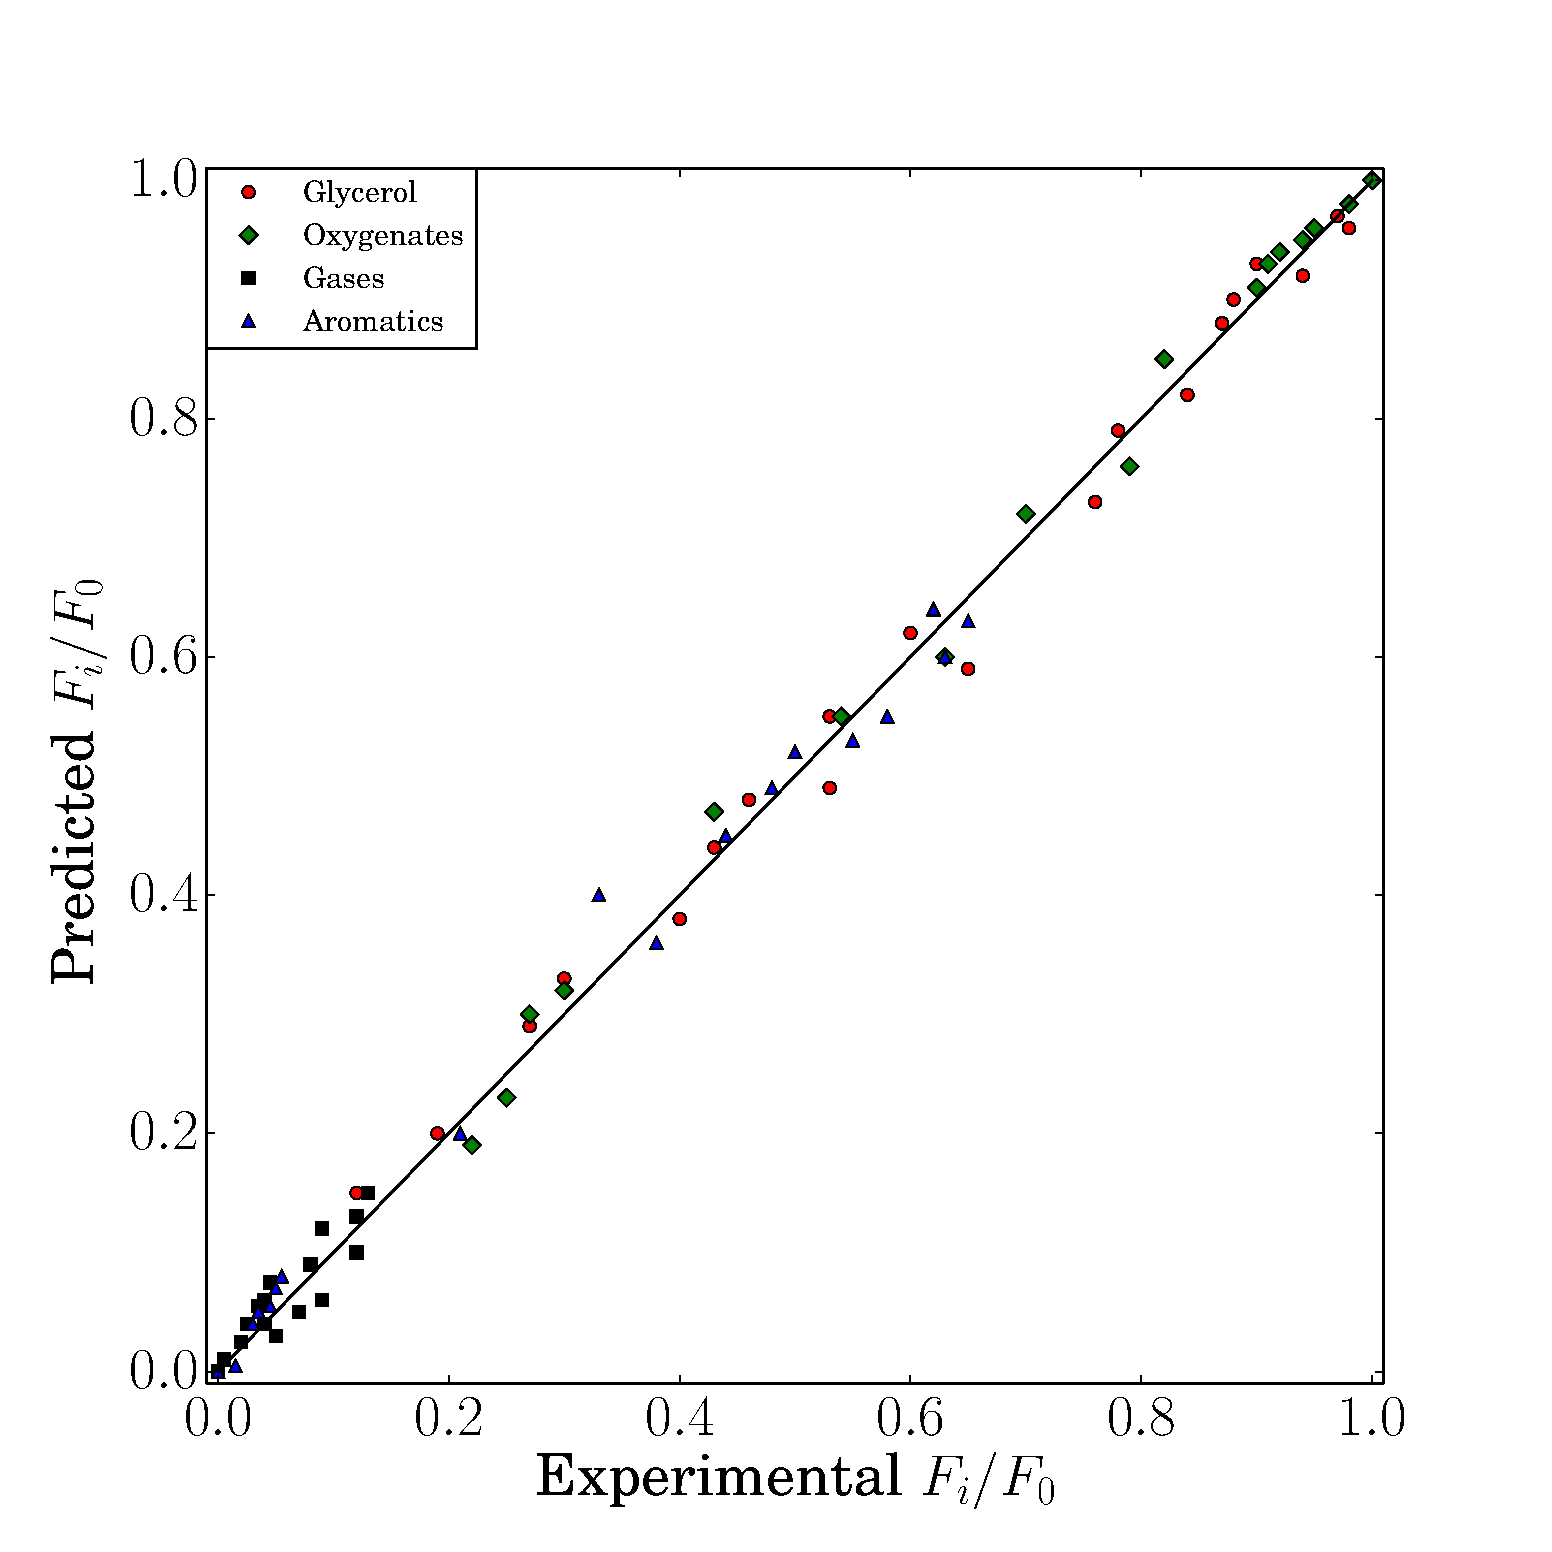
\includegraphics[width=0.85\textwidth]{Fig7.eps}
  \caption{Comparison of Experimental and Predicted Flow Rates}  \label{F_parity}
\end{figure}



\newpage
\begin{table}[h]
  \centering
  \caption{Product Distribution of GTH Conversion over Different Catalysts \cite{Xiao2016}} \label{T_products}
  \begin{tabular}{c c c c c c c c c c c}
    \toprule
    & H-ZSM-5    & Pd/H-ZSM-5 \\
    \midrule
    Glycerol   & 9.8        & 8.0       \\
    Oxygenates & 58.3       & 23.2      \\
    Gases      & 8.7        & 7.4       \\
    Aromatics  & 23.2       & 61.4      \\
    \bottomrule
  \end{tabular}
\end{table}

\begin{table}[h]
  \centering
  \caption{Reaction Rate Constants at 400 $^{\circ}$C; units of $k_i$, $mol$/($g_{cat}$ $\cdot$ h $\cdot$ $atm^{n_i}$)} \label{T_all_k}

  \begin{tabular}{c c c c c c c c c c c}
    \toprule
    & $R_1$      & $R_2$      & $R_3$      & $R_4$  \\
    \midrule
    $k_i$      & 0.278      & 0.923      & 0.045      & 0.741          \\
    \bottomrule
  \end{tabular}
\end{table}

\begin{table}[h]
  \centering
  \caption{GTH Conversion Reaction Network Summary} \label{T_Ea}
  \begin{tabular}{c c c c c c c c c c c}
    \toprule
    & $R_1$      & $R_2$      & $R_3$      & $R_4$  \\
    \midrule
    $n_i$      & 1          & 2          & 2          & 1        \\
    $E_{a_i}, kJ/mol$     & 105        & 121        & 147        & 125      \\
    $A_{i},10^7 mol/(g_{cat} \cdot h \cdot atm^{n_i})$     & 1.53        & 517        & 276        & 610      \\
    \bottomrule
  \end{tabular}
\end{table}





\end{document}

